%*******************************************************************************
% * Copyright (c) 2006-2013 
% * Institute of Automation, Dresden University of Technology
% * 
% * All rights reserved. This program and the accompanying materials
% * are made available under the terms of the Eclipse Public License v1.0 
% * which accompanies this distribution, and is available at
% * http://www.eclipse.org/legal/epl-v10.html
% * 
% * Contributors:
% *   Institute of Automation - TU Dresden, Germany 
% *      - initial API and implementation
% ******************************************************************************/

\documentclass[
  screen,          % print optimized version of the thesis, standard option
                  % alternative:
%  screen,        % makes the thesis better readable on screens (onesided, coloured links)
                  % use only 'print' OR 'screen'
                  % ATTENTION: 'screen' changes size of text area slightly. Always optimize document WITH
                  % 'print' option first for printing (size of graphics etc.) and convert afterwards
                  % in screen optimized version!
  listoffigures,  % includes list of figures
  listoftables,   % includes list of tables
  listoflistings, % includes list of listings
  abbrevations,   % includes index of symbols and abbrevations
  bibIfa,         % citation style (IfA standard), alternatives: bibNumeric, bibHarvard
  biber,          % bibliography backend, alternatives: bibtex, bibtex8, biber
  langEN         % define the language (default: langDE)
%  noIfaLogo,     % prevents the 'IfA' logo from being inculded in the header for the title page and abstract
%  a5paper        % switches to 'A5' paper size (this may only be used for Dissertations!!!)
]{ifathesis}

%***********************************
% General commands
%***********************************

\ifaThesis{Bachelor Thesis}                               % type of the thesis                
\ifaAuthor{Pablo Rodríguez Robles}                            % author of the thesis
\ifaAuthorBirthday{28.02.1996}                         % date of birth
\ifaAuthorBirthplace{León, Spain}             % place of birth
\ifaAuthorCourse{Aerospace Engineering}                          % study program
\ifaAuthorYearOfMatriculation{2014}                    % year of immatriculation
\ifaKeywords{Visual Servoing, Flying Robot, Quadrotor, Visual Navigation, GNC}    % Keywords included in pdf-file. Could be found e.g. by Windows file search.
\ifaTitleDE{Image Based Visual Servoing for Aerial Robot}       % geman title of the thesis
\ifaTitleEN{Image Based Visual Servoing for Aerial Robot}         % english title of the thesis
\ifaAbstractDE{example_files/00_abstract_de}           % a tex file containing the german abstract
\ifaAbstractEN{example_files/00_abstract_en__invalid}  % a tex file containing the german abstract
%\ifaAbbrev{content/abbrev.tex}                                          % a tex file containing the various abbreviations to include into the list of abbreviations (alternatively,
%\ifaUserListings{}                                    % a tex file containing additional listings to be printed (besides list of figures, tables, and/or listings)
%\ifaAcknowledegments{}                                % the acknowlegements for the thesis (usually only used for dissertation)
                                                       % these may also be defined in the text where they are first used)

% supervisors of the thesis (for dissertations, this can be used to indicate the reviewers)
\ifaSupervisorA{Dipl.-Ing. Chao Yao}
%\ifaSupervisorB{Dipl.-Ing. Arne Sonnenburg}
%\ifaSupervisorC{PD Dr.-Ing. Annerose Braune}
%\ifaSupervisorD{}
%\ifaSupervisorE{}

\ifaProfessor{Prof. Dr. techn. Klaus Janschek}         % supervising professor as indicated on the topic description
\ifaDayOfSubmission{27.03.2018}                        % the day the thesis is submitted
\ifaTopicDescriptionPDF{example_files/00_Aufgabenstellung.pdf} % a PDF file of the topic description
\ifaAppendix{example_files/appendix}                   % a tex file containing the appendix for the thesis

% Literaturverzeichnis angeben
\bibliography{bibliography}                            % a bib file containing the reference sources
\ifaBibliographyBeforeAppendix{false}	                 % print the bibliography before or after the appendix ('true' or 'false')
%\ifaAdditionalContributors{}                           % additional contributors to be included in the statement of authorship

%***********************************
% Special commands for dissertations
%***********************************

%\ifaDissertationStage{Pflichtexemplare}                      % stage of the dissertation ('Gutachten' or 'Pflichtexemplare')
%\ifaChair{}                                           % chair of the phd board
%\ifaDayOfDefense{}                                    % the day the dissertation was defended (only used in 'Pflichtexemplare' mode)
%\ifaIncludeBeforeTitlePage{}                          % include additional content before the title page (e.g. bastard title or impressum)
%\ifaIncludeAfterTitlePage{}                           % include additional content between title page and abstract (e.g. impressum or dedication)
%\ifaCV{}                                              % include a CV at the end of the document
%\ifaIncludeAtEndOfDocument{}                          % include additional content at the end of the document (e.g. to reach an even number of pages)


%***********************************
% The actual content of the thesis
%***********************************

\begin{document} 
	
	
% Chapter 0	
%!TEX root = ../thesis_master.tex
%**************************************************
% * Copyright (c) 2006-2013 
% * Institute of Automation, Dresden University of Technology
% * 
% * 
% * Contributors:
% *  	Institute of Automation - TU Dresden, Germany 
% *     	- initial API and implementation
% * 
% * Author:
% * 	Pablo Rodríguez Robles
% * 		- Author of this document
% * 	
%**************************************************


% Dieser Befehl setzt das Nomenklaturverzeichnis mit angegebener Breite für die erste Spalte
\printnomenclature[2.3cm]

% Falls das Abkürzungs- und Symbolverzeichnis ohne Nutzung des nomencl-Pakets 
% von Ihnen selber erstellt werden soll (z.B. in einer Tabelle), ersetzen Sie 
% einfach den /printnomenclature - Befehl durch eigenen Quellcode.

% In Ihrem Dokument können Sie dann bei jeder Verwendung einer Abkürzung oder 
% eines neuen Symbols diese/dieses kurz über den \nomenclature Befehl erklären 
% und dem Abkürzungsverzeichnis zur Verfügung stellen.

% Ein Beispiel für ein Symbol ("yx"):
%   \nomenclature[yx ]{$a_{BA}$}{Anteil der ausgegebenen Nullen}

% Ein Beispiel für eine Abkürzung ("ba"):
%   \nomenclature[ba ]{DIP}{Bildprozessor ("`Digital Image Processor"')}


%\input{content/chapter_00/00_abstract_de.tex}
%\input{content/chapter_00/00_abstract_en.tex}
%\input{content/chapter_00/00_Vorab.tex}

% Chapter 1
%!TEX root = ../../thesis_master.tex

%%%%%%%%%%
\chapter{Introduction}
\label{chap:introduction}
%%%%%%%%%%

%%%%%%%%%%
\section{Motivation and Background}
\label{sec:motivation-brackground}
%%%%%%%%%%

During the last decade, the use of Unmanned Aerial Vehicles (UAVs) has spread among very different applications. Flying robots can be very helpful to improve the way some tasks are already achieved by terrestrial platforms. For example, object transportation, environment mapping or surveillance. At the Institute of Automation Engineering\footnote{Technische Universität Dresden. Institut für Automatisierungstechnik. 01062 Dresden, Germany} of the Technical University of Dresden, a drone is being developed in cooperation with the Institute of Solid Mechanics\footnote{Technische Universität Dresden. Institut für Festkörpermechanik. 01062 Dresden, Germany} to investigate the use of flying robots in aerial manipulation.

\nomenclature[ba]{UAV}{Unmanned Aerial Vehicle}
\nomenclature[ba]{TUD}{Technische Universität Dresden}

When dealing with manipulation of objects, it is desired that the aerial robot adopts a certain pose with respect to the target before the manipulation process really starts. The present work deals with the development of a Visual Servoing (VS) control system that helps a quadrotor robot to acquire the desired pose by means of image data.

\nomenclature[ba]{VS}{Visual Servoing}

A monocular monochrome camera as well as an Inertial Measurement Unit (IMU) are planed to be the only available on board sensors. For the controller proposed the feedback is directly computed from image features rather than estimating the robot’s pose and using the pose errors as control input.

\nomenclature[ba]{IMU}{Inertial Measurement Unit}

Vision results to be a passive (in contrast to GPS) and cheap sensor (in contrast to LIDAR system). Visual odometry is very helpful to navigate in GPS denied environments like indoors, but its not appropriated to regulate the relative navigation of the vehicle with respect to a target.  

\nomenclature[ba]{LIDAR}{Light Detection and Ranging}

In order to integrate the visual servoing algorithm into the future modular robot system, the algorithm has been designed and tested on a under-actuated conventional quadrotor. The aerial robot is implemented within the ROS\footnote{\url{www.ros.org}} framework, where the visual servoing controller developed for this thesis is also integrated. Instead of using real hardware the complete system is simulated using Gazebo\footnote{\url{ www.gazebosim.org}}.

\nomenclature[ba]{ROS}{Robot Operative System}

%%%%%%%%%%
\section{Aims and Objectives}
\label{sec:aims-objectives}
%%%%%%%%%%

The aim of this work is to implement and test a VS control algorithm for a quadrotor, which could be later used by the HORUS (TODO: Add reference) project. This includes the review of the state of the art with regard to Visual Servoing, the design of a solution and a prototypical implementation with in the ROS framework and simulation with Gazebo of a test case.

The present thesis documents comprehensively the theoretical background, implementation details and results of the conducted work through the following structure. In Chapter \ref{chap:theory-state-art} the theoretical background and state of the art of Visual Servoing is presented. Chapter \ref{chap:srs-sa} gives a description of the system requirements as well as the system decomposition by Structure Analysis (SA) (see \cite{SA_Braune}). Chapter \ref{chap:system-design} describes the solution developed and the algorithms to be tested. Chapter \ref{chap:implementation} deals with the implementation, testing and validation. Finally, Chapter \ref{chap:results-conclusions} contains the final results and conclusions and Chapter \ref{chap:future-work} suggests future improvement and research paths.

\nomenclature[ba]{ROS}{Structure Analysis}

%Chapter 2
%!TEX root = ../thesis_main.tex

%%%%%%%%%%
\chapter{Theoretical Background and State of the Art}
\label{chap:theory-state-art}
%%%%%%%%%%

\section{Visual Servoing Theoretical Basics}

In this section the theoretical basic background of visual servo controllers is briefly discussed. It is usual in the literature to take \cite{chaumette_visual_2006} and \cite{chaumette_visual_2007} as the main reference when it comes to the theoretical setup of the discipline. As a result, the following description is completely based on these popular sources\footnote{The interested reader should visit the Lagadic research group home page (\url{http://www.irisa.fr/lagadic}), pioneers in the area.}.

Visual Servoing is defined in the literature as the use of computer vision data to control the motion of a robot. The image data comes from a camera, which can observe the robot fixed in the space or moving with the robot. The latter approach is know as eye-in-hand Visual Servoing and is the selected one for the case of this work.

Visual servo controllers accomplish their task of reaching a certain pose by trying to minimize the following error $\bm{e}(t)$

\begin{equation}
\bm{e}(t) = \bm{s}(\bm{m}(t), \bm{a}) - \bm{s}^\ast
\label{eq:vs-th-1}
\end{equation}

Here, $\bm{m}(t)$ is a set of image measurements (e.g. the image coordinates of the interest points or the image centroid of an object), that is, information computed from the image data. With the help of these measurements a vector of $k$ visual features, $\bm{s}(\bm{m}(t), \bm{a})$ is obtained, in which $\bm{a}$ is a vector containing different camera parameters. In contrast, $\bm{s}^\ast$ defines a set of desired features.

For the present case, where the target is not moving,  $\bm{s}^\ast$ and the changes in $\bm{s}$ depend only on the camera motion.

There exist two main variants of Visual Servoing depending on how the features vector $\bm{s}$ is defined. On the one hand, Image Based Visual Servoing (IBVS) takes as $\bm{s}$ a set of features already available within the image data (TODO it can be seen as a control of the features in the image plan such that moving the features to a goal configuration implicitly results in the task being accomplished \cite{espiau_1992}). On the other hand, Position Based Visual Servoing (PBVS) considers for $\bm{s}$ a set of 3D parameters that must be estimated from the image data (TODO: Add that it is a cartesian motion planing problem).

\nomenclature[ba]{IBVS}{Image Based Visual Servoing}
\nomenclature[ba]{PBVS}{Position Based Visual Servoing}

Using the PBVS approach leads to the necessity of camera calibration and estimation of the flying robot pose (TODO: Add reference or a bit more of information), these are two big disadvantages for the application intended in this work. On the other side, IBVS needs no camera calibration and allows the robot to achieve the pose desired without any pose estimation process.

A simple velocity controller can be arranged in the following way. Let $\bm{v}_c = (v_c, \bm{\omega}_c)$ be the spatial velocity of the camera, with $v_c$ the instantaneous linear velocity of the origin of the camera frame and $\bm{\omega}_c$ the instantaneous angular velocity of the camera frame, as a result we can express the temporal variation of the features vector as

\begin{equation}
\dot{\bm{s}} = \bm{L_s} \bm{v}_c
\label{eq:vs-th-2}
\end{equation}
  
Where $\bm{L_s} \in \mathbb{R}^{k \times 6}$, the feature Jacobian, acts as iteration matrix relating the camera velocity and the change in the visual features.

The time variation of the error to be minimized can be obtained by combining \ref{eq:vs-th-1} and \ref{eq:vs-th-2}

\begin{equation}
\dot{\bm{e}} = \bm{L_e} \bm{v}_c
\label{eq:vs-th-3}
\end{equation}

with $\bm{L_e} = \bm{L_s}$. The input for such a controller is the camera velocity  $\bm{v}_c$, which, using \ref{eq:vs-th-3}, we can set in such a way that an exponential decrease of the error is imposed (i.e. $\dot{\bm{e}} = - \lambda \bm{e}$) 

\begin{equation}
\bm{v}_c = - \lambda \bm{L_e}^+ \bm{e}
\label{eq:vs-th-4}
\end{equation}

Here, $\bm{L_e}^+ \in \mathbb{R}^{k \times 6}$ is the Moore-Penrose pseudoinverse of $\bm{L_e}$. It is computed as $\bm{L_e}^+ = (\bm{L_e}^T \bm{L_e})^{-1} \bm{L_e}^T$, provided that $\bm{L_e}$ is of full rank 6. Imposing this condition leads to $\| \dot{\bm{e}} - \lambda \bm{L_e}^T \bm{L_e} \bm{e} \|$ and $\| \bm{v}_c \|$ being minimal. Note that for the special case of $k=6$, if $\bm{L_e}$ is nonsingular, it is possible to obtain a simpler expression using the matrix inversion $\bm{v}_c = - \lambda \bm{L_e}^{-1} \bm{e}$.

When implementing real systems it is not possible to know perfectly either $\bm{L_e}$ or $\bm{L_e}^{+}$. Thus, an approximation of these two matrices is introduced, noted with the symbol $\widehat{\bm{L_e}}$ for the approximation of the error interaction matrix and $\widehat{\bm{L_e}^+}$ for the approximation of the pseudoinverse of the interaction matrix. Inserting this notation in the control law we obtain

\begin{equation}
\bm{v}_c = - \lambda \widehat{\bm{L_e}^+} \bm{e}
\label{eq:vs-th-5}
\end{equation}

Once the basic appearance of a visual servo controller has being presented, the goal is to ask the following questions: How should $\bm{s}$ be chosen?  What is the form of $\bm{L_s}$? How should we estimate $\widehat{\bm{L_e}^+}$?

In the simplest approach, the vector $\bm{s}$ is selected as a set of image-plane points, where $\bm{m}$ are the set of coordinates of these  image points and $\bm{a}$ the camera intrinsic parameters. Later in this work, a more complex definition for the image features vector $\bm{s}$ will be chosen.

\subsection*{The Interaction Matrix}

The camera image capture is a procedure which projects a 3D point from its coordinates in the camera frame, $\bm{X} = (X, Y, Z)$, to a 2D image point with coordinates $\bm{x} = (x, y)$. From this geometry we have

\begin{equation}
\begin{cases}
x = X/Z = (u - c_u) / f \alpha \\
y = Y/Z = (v - c_v) / f
\end{cases}
\label{eq:vs-th-6}
\end{equation}

where $\bm{m} = (u, v)$ gives the coordinates of the image point in pixel units, and $\bm{a} = (c_u, c_v, f, \alpha)$ is the set of camera intrinsic parameters: $c_u$ and $c_v$ are the coordinates of the principal point, $f$ is the focal length, and $\alpha$ is the ratio of the pixel dimensions. In this case, we take as feature the image point, thus $\bm{s} = \bm{x} = (x, y)$.

Taking the time derivative of the projection equations \ref{eq:vs-th-6}, we obtain

\begin{equation}
\begin{cases}
\dot{x} = \dot{X}/Z - X\dot{Z}/Z^2 = (\dot{X} - x \dot{Z})/Z \\
\dot{y} = \dot{Y}/Z - Y\dot{Z}/Z^2 = (\dot{X} - y \dot{Z})/Z
\end{cases}
\label{eq:vs-th-7}
\end{equation}

The velocity of the 3D point can be related to the spatial velocity of the camera using the equation for the velocity in a non-inertial reference frame

\begin{equation}
\dot{\bm{X}} = - \bm{v}_c - \omega_c \times \bm{X} \Leftrightarrow
\begin{cases}
\dot{X} = - v_x - \omega_y Z + \omega_z Y \\
\dot{Y} = - v_y - \omega_z X + \omega_x Z \\
\dot{Z} = - v_z - \omega_x Y + \omega_y X 
\end{cases}
\label{eq:vs-th-8}
\end{equation}

Introducing \ref{eq:vs-th-8} in \ref{eq:vs-th-7}, and grouping terms we can write

\begin{equation}
\begin{cases}
\dot{x} = - v_x / Z + x v_z / Z + xy \omega_z - (1 + x^2) \omega_y + y \omega_z \\
\dot{y} = - v_y / Z + y v_z / Z + xy \omega_z - (1 + y^2) \omega_x + x \omega_z 
\end{cases}
\label{eq:vs-th-9}
\end{equation}

using matrix notation

\begin{equation}
\dot{\bm{x}} = \bm{L_x} \bm{v}_c
\label{eq:vs-th-10}
\end{equation}

where the interaction matrix that relates the camera velocity $\bm{v}_c$ to the velocity of the image point $\dot{\bm{x}}$ is

\begin{equation}
\bm{L_x} = 
\begin{bmatrix}
\frac{-1}{Z} & 0  & \frac{x}{Z}  & xy  &  -(1+x^2) & y \\ 
0 & \frac{-1}{Z} &  \frac{y}{Z} & 1+y^2 &  -xy & -x
\end{bmatrix}
\label{eq:vs-th-11}
\end{equation}

In Equation \ref{eq:vs-th-11}, the value $Z$ corresponds to the depth of the point relative to the camera frame. As a result, any Visual Servoing scheme using this form of the interaction matrix must provide an estimation of this value. Furthermore, the camera intrinsic parameters are necessary to compute $x$ and $y$. Therefore, it is not possible to use directly $\bm{L_x}$, but an approximation $\widehat{\bm{L_x}}$ is to be used.

\subsection*{Approximation of the Interaction Matrix}

When the current depth $Z$ of each point is known, there is no need of approximation and $\widehat{\bm{L_e}^+} = \bm{L_e}^+$ for $\bm{L_e} = \bm{L_x}$ can be used. However, this approach requires the estimation of $Z$ for all iterations of the scheme control (see \cite{hutchinson_1996}), which may be conducted by means of pose estimation methods.

A second alternative is to use $\widehat{\bm{L_e}^+} = \bm{L_{e^\ast}}^+$, where $\bm{L_{e^\ast}}$ is the value of $\bm{L_{e}}$ for the desired position ($\bm{e} = \bm{e}^\ast = 0$) (see \cite{espiau_1992}). Here, the depth parameter only needs to be estimated once for every point.

\section{State of the Art}

\subsection{Visual Servoing for Aerial Robots}

In this section the literature on the use of Visual Servoing to control de translation of aerial robots is analyzed. The focus of this review is on the IBVS approach, where image feature errors between the current and target image are mapped to actuator inputs through the inverse of the Jacobian matrix. The different approaches discus the alternatives on feature selection, Jacobian matrix construction and different control strategies to make the error converge to zero, and with it, the relative pose between UAV and target object will converge to the desired one.

One of the problems of the classical formulation of IBVS is the necessity to estimate the depth of each of the features. In the past several approaches have been taken to cope with this problem, such as: partial pose estimation (see \cite{malis_2_1999}), adaptive control (see \cite{Papanikolopoulos}) or estimation of the Jacobian using quasi-Newton methods (see \cite{Piepmeier}). An alternative is to use a hybrid control approach by treating rotational and translational control separately. However, it is important to bear in mind that due to the under-actuated dynamics of an usual 4 DOF quadrotor, it is only possible to control the three linear velocities and the yaw (rotational) speed. While the other two rotational speeds, roll and pith, are used to move the thrust vectors of the propellers and thus generate movement on the horizontal plane.

Most of the Visual Servoing methods have been developed for serial manipulators. For this kind of robot, a low-level actuator is usually employed to compensate the dynamic behavior of the system, making possible to control it with velocity commands as a first order system. For a full-dynamics quadrotor model accounting for aggressive maneuvers this is not at all the case, since it is a fourth order system. Thus, other strategies are usually considered to control such a robot (see\cite{Mellinger}).

% \cite{guenard_2008}

Uses 

\subsection{Visual Servoing for Aerial Manipulators}

% (TODO: Tabla con tipo de vehículo, dofs del brazo, tipo de control, tipo de cámara, feature)
% (TODO: Very important). Vision is a passive and cheap sensor. Visual odometry does no provide the ability to control the vehicle with respect to a specific target. So not useful for manipulation tasks.

% (TODO: Para introducción)
% Particularly, rotary-wing vehicles possess the capability of holding stationary and therefore passing through cumbersome spaces. This makes them relevant candidates for applications such as sensing and surveillance,
%Aerial manipulation systems can be used to do this dangerous, difficult or expensive work in locations that can only be reached while flying. Examples are maintenance and inspection of tall buildings, power lines, chemical plants, bridges or work in mountain areas. Another example is manipulation and in-situ measurements during nuclear, chemical or biological disas- ters and accidents. 
% (TODO: No habla de visión, solo fuentes que usan robots para contruir estructuras. Todos usan indoor y control externo) Successful aerial manipulation and building of complex structures have been presented in [1], [2] and [3].
% (TODO: Important. Si brazo usado para compensar under-actuation, por qué usar ambos?)Multirotors, and in particular quadrotors such as the one used in this work, are underactuated platforms. That is, they can change their torque load and thrust/lift by altering the velocity of the propellers, with only four degrees-of-freedom (DOF), one for the thrust and three for the torques. But, as shown in this paper, the attachment of a manipulator arm to the base of the robot can be seen as a strategy to alleviate underactuation allowing UAM to perform complex tasks.


% (TODO: Main reference to image moments [17, mebarki_exploiting_2013].)

In this section a perspective of Visual Servoing applied to aerial manipulators is presented. The main literature is analyzed and some of the common characteristics of the approaches followed by them are highlighted.

% Aerial gripping

Some publications related to the University of Pennsylvania GRASP Laboratory\footnote{\url{https://www.grasp.upenn.edu}}  (see \cite{thomas_toward_2014} and \cite{thomas_visual_2016}) have studied the vision-based localization and servoing of quadrotors in grasping and perching tasks. However, the emphasis of these publications lays on the generation of dynamically-feasible trajectories in the image space, thus second order system control is performed instead of the most common kinematic control strategy. These vehicles are not manipulators in the sense of the rest of the approaches presented in this section, since the main task here is hanging from structures and grasping targets by means of aggressive, thus dynamical, maneuvers. In addition to that, the actuator used is not a high-DOF actuator, but a 1 DOF gripper.  

In the last years, a concrete aerial manipulator architecture has been popularized, for example in the context of the European projects ARCAS\footnote{\url{http://www.arcas-project.eu}} and AEROARMS\footnote{\url{http://www.arcas-project.eu}}. These aerial manipulators have usually the task of collecting an structural element from its initial position and fly it to a final position, where the element is used to assemble a strut structure. The main configuration of such a robot is an under-actuated rotary-wing aircraft (usually a quadrotor) and a robotic manipulator arm. Different degrees of freedom (DOF) are used for the arm and different camera placements are considered.
 
  \nomenclature[ba]{DOF}{Degree of Freedom}
 
 The usual implementation considers the simultaneous control (at the velocity level) of the mobile platform (i.e. quadrotor) and the manipulator for such a grasping task. Since the sum of the 4 DOF of a quadrotor plus the multiple-DOF of a serial manipulator leads to a redundant system, the possibility of choosing degrees of freedom is used to realize different subtasks (e.g. joint reaching prevention). The Visual Servoing controller chosen generates velocity inputs both for the manipulator joints (i.e. $\bm{\dot{q}}$) and for the quadrotor (i.e. translational velocity $\bm{v}$ and rotational velocity $\omega_z$). The use of a weighted pseudo-inverse allows to favor the control of the mobile platform when the distances to the target are bigger and increase the manipulator use when it is close to the target.
 
 % \cite{mebarki_image-based_2014}
 
 \cite{mebarki_image-based_2014} propose a quadrotor equipped with a 5 DOF arm. Traditional Visual Servoing distinguishes between two different classes of camera configuration: eye-to-hand (fixed in the workspace) and eye-on-hand (mounted on the mobile platform). In this paper a new configuration for the camera is presented, called onboard-eye-to-hand, i.e. the camera is placed on-board of the robot while it observes the manipulator. In this way, the manipulator can accomplish large rotations while the target is not left out of the camera field of view, as happens in the eye-in-hand configuration. Furthermore, for the case of eye-in-hand configuration, during assembly tasks the manipulator end-effector can contact or impact with objects and damage or obstruct the camera. Thanks to the onboard-eye-to-hand camera configuration the paper is able to introduce a variation of the IBVS approach, called Self Visual Servoing (SVS). Where the error nullified comes directly form the image itself (hence the adjective self) an there is no need for a target image. The servo controller implemented has two different tasks. The main task is position the feature points at a target position on the target object and the second one the end-effector motion. Error formulation decouples both tasks and a wighted pseudo-inverse is used to provide a different gain for the arm joints rates $\bm{\dot{q}}$ and for the UAV velocities $\bm{v}$ and $\omega_z$.
 
 \nomenclature[ba]{SVS}{Self Visual Servoing}
 
 % \cite{mebarki_exploiting_2013}
 % \cite{mebarki_cross-coupled_2014}
 
 The image moments as features for the Visual Servoing are proposed in \cite{mebarki_exploiting_2013} for the previous system. Furthermore, aerial manipulators have to cope with the change of the center of mass during flight due to the effect of suspended loads \cite{palunko_2012}. To achieve this behavior, low-level attitude controllers are usually designed to compensate this effects using Cartesian impedance control \cite{lippiello_impedance_2012} or adaptive control. To this end, the system includes a controller to reduce dynamic effects by vertically aligning the arm center of gravity to the multirotor gravitational vector, along with one that keeps the arm close to a desired configuration of high manipulability and avoiding arm joint limits. In \cite{mebarki_cross-coupled_2014}, the author completes the robot with a nonlinear low-level controller that thanks to a integral  approach allows the inclusion of the dynamic coupling of the UAV and the robotic arm, while the control of the system through the velocities provided by the IBVS high-level is maintained.
 
% \cite{danko_evaluation_2014}

In this case the source (see \cite{danko_evaluation_2014}) includes as host a gantry used to emulate an UAV and a 6 DOF manipulator with an end-effector mounted camera (i.e. eye-in-hand). Coordination of redundant degrees of freedom by means of partitioned control. Visual servoing is used to drive the end-effector pose relative to a target thanks to the use of feature points and their desired positions.

% \cite{lippiello_hybrid_2016}
% Uses Gazebo for simulations

\cite{lippiello_hybrid_2016} uses a hybrid-control framework the main benefits of both IBVS and PBVS schemes to control a octorotor with a 6 DOF arm. Kinematic redundancy of the end-effector is used to accomplish secondary tasks and lead by a hierarchical task-composition algorithm, in conjunction with a smooth activation mechanism for the tasks.

% \cite{laiacker_high_2016}


DLR's work within ARCAS project \cite{laiacker_high_2016} uses of an helicopter and a 7 DOF manipulator. The helicopter is a bigger robot when compared to the rest of the systems, with more than 1 m from manipulator to center of gravity. Influence of the arm movement is significant to the helicopter flight and is actively compensated by the robot controller by means of a coordinated control of both elements. The paper discusses performance and accuracy in aerial manipulation, where the time it takes between the measurement of a position difference and its compensation using the manipulator or the flying platform is the main factor. Additionally, the work presents a multi-marker approach to compensate occlusion of the target marker by the manipulator derived of the onboard-eye-to-hand camera configuration.


% \cite{kim_vision-guided_2016}
% (TODO: \cite{kim_vision-guided_2016} contains signal flow char for image processing and IBVS)

A combination of kinematic and dynamic models to develop a passivity-based adaptive controller which can be applied on both position and velocity control is proposed in \cite{kim_vision-guided_2016}. Position control is used for waypoint tracking and landing, while velocity control is triggered for target servoing. The robot is a quadrotor with a 3 DOF arm and an eye-in-hand camera. The work uses IBVS with image moments as visual features and tries to solve two problems of the method when applied to aerial manipulators (under-actuated system). Firstly, movements of the manipulator produce movement of the camera, thus making probable that the target object is taken out of its field of view. For this reason a fisheye camera is used. Secondly, the under-actuation of the robot is corrected introducing a image modification method. Velocity weighting of the Jacobian matrix in accordance of the situation is used for the simultaneous control of UAV and manipulator.

% \cite{santamaria-navarro_uncalibrated_2017}
% Uses Gazebo

% (TODO: ARCAS bot [santamaria-navarro_uncalibrated_2017] is called Kinton, avaible on the internet). 

In \cite{santamaria-navarro_uncalibrated_2017} redundant manipulation and hierarchical control law are combined with a new variation of the IBVS that does not need the camera parameters. The system establishes as primary task the avoidance of obstacles, as well as several secondary tasks. The visual servo strategy is used to drive the arm end-effector to a desired position and orientation by using a camera attached to it. The configuration used is a 4 DOF quadrotor and equipped with a 6 DOF robotic arm. In the common IBVS approaches, Jacobian or interaction matrix, which relates the camera velocity with the image feature velocities, depends on a priori knowledge of the intrinsic camera parameters. The paper presents a variation of IBVS called Uncalibrated IBVS, the approach uses the barycenter of the features as control points. The method recovers the coordinates of these control points and also the camera focal length, with this data a new formulation of the Jacobian is constructed. The system also compensates by means of a hierarchical algorithm the position of the manipulator.

\begin{table}[]
	\centering
	\caption{My caption}
	\label{my-label}
	\begin{tabular}{|l|l|l|l|l|l|l|}
		\hline
		Reference                                                       & Vehicle    & Manipulator's DOF & Camera configuration & VS Type           & Visual feature                                   & Comment                                                            \\ \hline
		\cite{thomas_toward_2014} and \cite{thomas_visual_2016} & quadrotor  & 1                 & eye-in-hand          & IBVS              & Cylinder parameters                              & agressive maneuvers                                                \\ \hline
		\cite{mebarki_image-based_2014}                             & quadrotor  & 5                 & onboard-eye-to-hand  & SVS               & points (no target)                               & -                                                                  \\ \hline
		\cite{mebarki_exploiting_2013}                              & quadrotor  & 5                 & onboard-eye-to-hand  & SVS               & perspective projection image moments (no target) & -                                                                  \\ \hline
		\cite{mebarki_cross-coupled_2014}                           & quadrotor  & 5                 & onboard-eye-to-hand  & SVS               & points (no target)                               & low-lever controller for dynamic coupling robot-arm                \\ \hline
		\cite{danko_evaluation_2014}                                & grantry    & 6                 & eye-in-hand          & IBVS              & points                                           & gantry used to emulate an UAV                                      \\ \hline
		\cite{lippiello_hybrid_2016}                                & octortor   & 6                 & onboard-eye-to-hand  & Hybrid VS         & points                                           & hierarchical task-composition algorithm, smooth task activation    \\ \hline
		\cite{laiacker_high_2016}                                   & helicopter & 7                 & onboard-eye-to-hand  & IBVS              & points                                           & discusses performance and accuracy, multi-marker approach          \\ \hline
		\cite{kim_vision-guided_2016}                               & quadrotor  & 3                 & eye-in-hand          & IBVS              & corrected perspective projection image moments   & adaptive controller for both position and velocity, fisheye camera \\ \hline
		\cite{santamaria-navarro_uncalibrated_2017}                 & quadrotor  & 6                 & eye-in-hand          & Uncalibrated IBVS & blobs' barycenters                               & hierarchical task-composition algorithm                            \\ \hline
	\end{tabular}
\end{table}



 

%Chapter 3
%!TEX root = ../../thesis_master.tex

%%%%%%%%%%
\chapter{Software Requirements Specification and Structured Analysis}
\label{chap:srs-sa}
%%%%%%%%%%

This chapter deals with the Software Requirement Specification (SRS) \cite{IEEE8301998} and the Structured Analysis \cite{SA_Braune} of the system developed in this work. Thanks to these two procedures, the objectives that the system must fulfill and a decomposition of it into different functions are stated. This leads to a complete definition of the system.

\nomenclature[ba]{SRS}{Software Requirement Specification}

The purpose of this work is to design a Visual Servoing controller to provide an under-actuated aerial robot the commands necessary to reach a desired pose with respect to a target object.

% TODO: Previously:

%The visual servo controller developed is to be integrated into the hector\_quadrotor\footnote{\url{http://wiki.ros.org/hector_quadrotor}} (see \cite{2012simpar_meyer}), an under-actuated aerial robot equipped with a monocular monochrome camera pointing downwards.

The visual servo controller developed is to be integrated into the HORUS aerial manipulator, a fully-actuated aerial robot equipped with a monocular monochrome camera pointing downwards.

% TODO: Reference for HORUS


%%%%%%%%%%
\section{Software Requirements Specification}
\label{sec:srs}
%%%%%%%%%%

In this section, the Software Requirement Specification \cite{IEEE8301998} for the visual servo controller developed in this thesis is presented. The use of SRS helps to define the system that is being designed, tracking continuously that the product developed satisfies the needs of the user. Only when every requirement stated therein is fulfilled the implementation would be completed.

%%%%%%%%%%
\subsection{Product Perspective}
\label{sec:product-perspective}
%%%%%%%%%%

The VS controller is to be used with an aerial robotic system based on the ROS framework. From the perspective of the robotic system, the VS controller subsystem will appear as a ROS node which publishes control commands through a ROS topic to the rest of the system.

% TODO: Previously:

%The aerial robotic system used is the hector\_quadrotor\footnote{\url{http://wiki.ros.org/hector_quadrotor}} model (see \cite{2012simpar_meyer}). (TODO: Add diagram).

The aerial robotic system used is the HORUS aerial manipulator developed at the Institute of Automation Engineering of the TUD.

% TODO: Reference for HORUS.

% TODO: Previously: "The output of the subsystem are the control inputs of the aerial robot system, a kinematic control is adopted, being this inputs the linear velocities of the vehicle and its yaw angular velocity."

The subsystem developed here is to interact with the camera hardware of the robot, a monocular monochrome camera pointing downwards. The output of the subsystem are the control inputs of the aerial robot system, a kinematic control is adopted, being this inputs the linear and angular velocities of the vehicle. These inputs interact with the already implemented inner control loop for the attitude in the robotic system and are the main input for the outer control loop, the one in charge of the translation.

% TODO: Add table with the hardware.

% TODO: State more accurately the how the inner and outer control loops interact with the attitude and position control.

% TODO : Sketch with the different control loops.

With the help of the visual servo controller, the robot is able to achieve a desired pose with respect to a target using only the visual information provided by the camera and with no pose computation involved.

%%%%%%%%%%
\subsection{User Characteristics}
\label{sec:user-characteristics}
%%%%%%%%%%

The product developed in this thesis will be used as part of a ROS-based system, thus the expected user is a designer willing to implement an Image Based Visual Servoing control strategy for his robotic system. The user should be familiarized with the ROS framework and the system will need the structure and interfaces of any standard ROS product.

%%%%%%%%%%
\subsection{Assumptions and Dependencies}
\label{sec:assumptions-dependencies}
%%%%%%%%%%

The software  has been tested on the following platform. Forward or backward support is not guaranteed on a different set-up.

\begin{itemize}
	\item ROS version: ROS Indigo\footnote{\url{http://wiki.ros.org/indigo}}
	\item Operating System: Ubuntu 14.04\footnote{\url{http://releases.ubuntu.com/14.04/}} Trusty Tahr, 64 bit
\end{itemize}

%%%%%%%%%%
\subsection{Functional Requirements}
\label{sec:functional-requirements}
%%%%%%%%%%

The functional requirements describe what the system must do to complete the overall task:

\begin{itemize}
	\item F1: \emph{Compute desired visual features}. For the desired pose with respect to the target, compute a vector of image features from the target. 
	
	\item F2: \emph{Compute current visual features}. For the current pose, compute a vector of image features from the target. 
	
	\item F3: \emph{Compute feature error}. Compute the difference between the desired current feature vector and the desired feature vector to be used as error for the control law.		
	
	\item F3: \emph{Give visual servoing control input}. Control input based on image data so that the aerial robot achieves the desired pose with respect to the target. Control based on the error between current and desired image features, no pose estimation.
	
	\item F5: \emph{Tell user when the target pose is achieved}. The system must be able of telling the user whether the target pose has been already achieved or not.
	
\end{itemize}

%%%%%%%%%%
\subsection{Other Requirements}
\label{sec:other-requirements}
%%%%%%%%%%

\begin{itemize}
	\item A1: All components are working reliably.
	\item A2: The software is sufficiently fast, modular and modifiable.
	\item A3: The implementation is transparent and comprehensible.
	\item A4: Control inputs must provide stable and smooth flight maneuvers.
	\item A5: Robot must be able to start from different initial positions.
	\item A6: Algorithm must be fast enough to allow real time control of the aerial robot.
	\item A7: The implementation should follow the style guide of ROS \cite{ROS_Style}.
\end{itemize}

%%%%%%%%%%
\subsection{General Constraints}
\label{sec:general-constraints}
%%%%%%%%%%

\begin{itemize}
	\item The environment must be sufficiently illuminated for the camera to work.
	\item The observed object must be planar and continuous and provided to the program as a binary image obtained by segmentation algorithms.
	\item The target pose must be provided by a sufficient number of features.
	\item The target must be always in the filed of view of the camera, so features can be extracted an control input computed.
	\item Testing computer is a MacBook Pro\footnote{\url{https://everymac.com/systems/apple/macbook_pro/specs/macbook-pro-core-i5-2.7-13-early-2015-retina-display-specs.html}} (Early 2015) with 2.7 GHz Intel Core i5 processor, 8 GB 1867 MHz DDR3 memory and Intel Iris Graphics 6100 1536 MB graphics. Linux OS is run using Oracle VM VirtualBox\footnote{\url{www.virtualbox.org}} (Version 5.1.14 r112924) with 5 GB base memory and two processors.
\end{itemize}

\nomenclature[ba]{OS}{Operative System}

%%%%%%%%%%
\section{Structured Analysis}
\label{sec:sa}
%%%%%%%%%%

The Structured Analysis \cite{Janschek2011} is a formal method to describe relationships of functional type in complex processes. In order to do that, it views the system from the perspective of data flowing through it. The Structured Analysis is a top-down model, meaning that it analyses the system data flows through successive decomposition. The result of the Structured Analysis of a system is a set graphical diagrams representing the different processes or functions applied to the data and the outputs stored by the system.

% TODO: Continue with next paragraph:

% In this work, the system has been divided in ... levels ...

%%%%%%%%%%
\subsection{Context Diagram}
\label{sec:context-diagram}
%%%%%%%%%%

The context diagram shows the interfaces between the system developed in this work and its environment.

\begin{figure}[h]
	\centering
	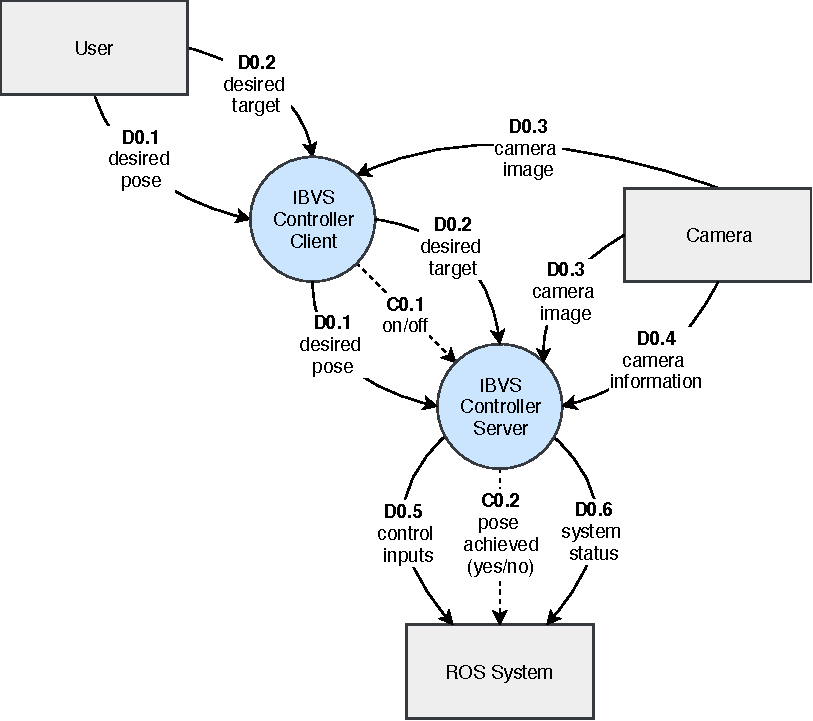
\includegraphics[width=0.8\textwidth]{content/chapter_03/images/sa_diagram_01.pdf}
	\caption{Context Diagram}
	\label{fig:sa_diag_01}
\end{figure}

\pagebreak

%%%%%%%%%%
\subsection{Level A: IBVS Controller}
\label{sec:level-A}
%%%%%%%%%%

Level A is the first level below the context diagram and contains the main functions (defined in Section \ref{sec:functional-requirements} as F1, F2, F3, F4 and F5) of the system developed, the \textit{IBVS Controller}. In Figure \ref{fig:sa_diag_02} a Data Flow Diagram (DFD) is used to describe the interaction between data and processes. A Data Flow Diagram \cite{Janschek2011} is a decomposition of the system developed resultant of the subjective perspective of the design engineer about it.

\nomenclature[ba]{DFD}{Data Flow Diagram}
\nomenclature[ba]{DD}{Data Dictionary}

\begin{figure}[!htb]
	\centering
	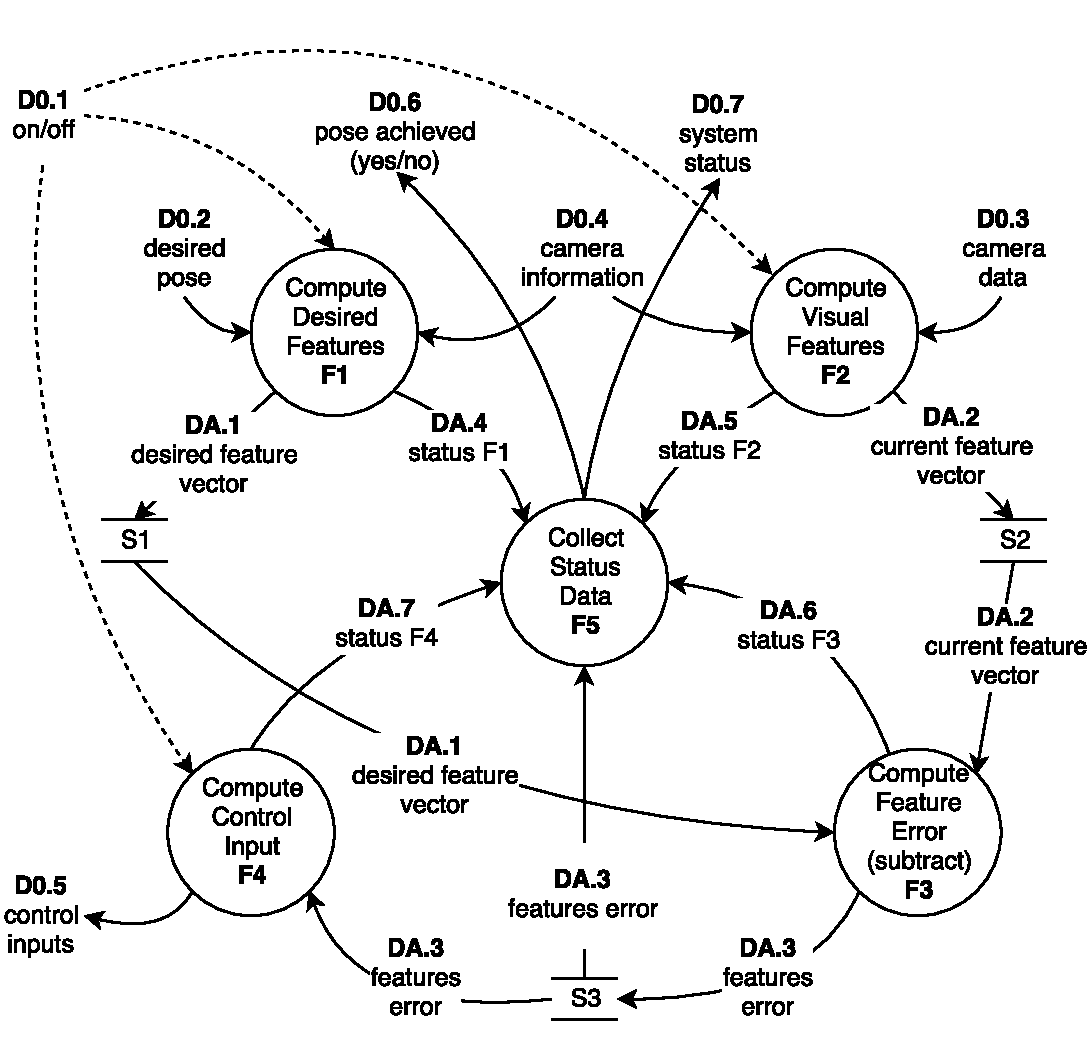
\includegraphics[width=\textwidth]{content/chapter_03/images/sa_diagram_02.pdf}
	\caption{Data Flow Diagram - Level A}
	\label{fig:sa_diag_02}
\end{figure}

\pagebreak

Table \ref{tab:DD-LA} contains the Data Dictionary for the DFD of Level A. The Data Dictionary \cite{Janschek2011} is a detailed representation of all data flows involved in a Data Flow Diagram. Where $D = \text{data flow}$ and $C = \text{control flow}$.

\begin{table*}[!htb]
	\centering
	\begin{tabular}{lll}
		\toprule
		Flow & Type & Description \\
		\midrule
		D0.1 & C & User input to start or stop the system \\
		D0.2 & D & User defined desired pose w.r.t. the target \\
		D0.3 & D & Camera image data \\
		D0.4 & D & Camera information (sensor data, camera model, etc.) \\
		D0.5 & D & Velocity control inputs in camera robot's bod \\
		D0.6 & C & Information about pose achieved or not \\
		D0.7 & D & System status presented to the user \\
		\midrule
		DA.1 & D & Feature vector for desired pose \\
		DA.2 & D & Current feature vector from camera image data \\
		DA.3 & D & Features error vector used for control law \\
		DA.4 & D & System status from process F1 \\
		DA.5 & D & System status from process F2 \\
		DA.6 & D & System status from process F3 \\
		\midrule
		S1 & Datastore & Desired feature vector \\
		S2 & Datastore & Current feature vector \\
		S3 & Datastore & Feature error vector \\
		\bottomrule
	\end{tabular}
\caption{Data Dictionary for Level A}
\label{tab:DD-LA}
\end{table*}

\pagebreak

%%%%%%%%%%
\subsection{Level B1: Compute Desired Visual Features}
\label{sec:level-B1}
%%%%%%%%%%

% TODO: In case of design alternative, this level may change. Desing variants are named with letters.

Figure \ref{fig:sa_diag_03} contains the Data Flow Diagram that describes the inner work of the process \textit{F1: Compute desired visual features}.

\begin{figure}[!htb]
	\centering
	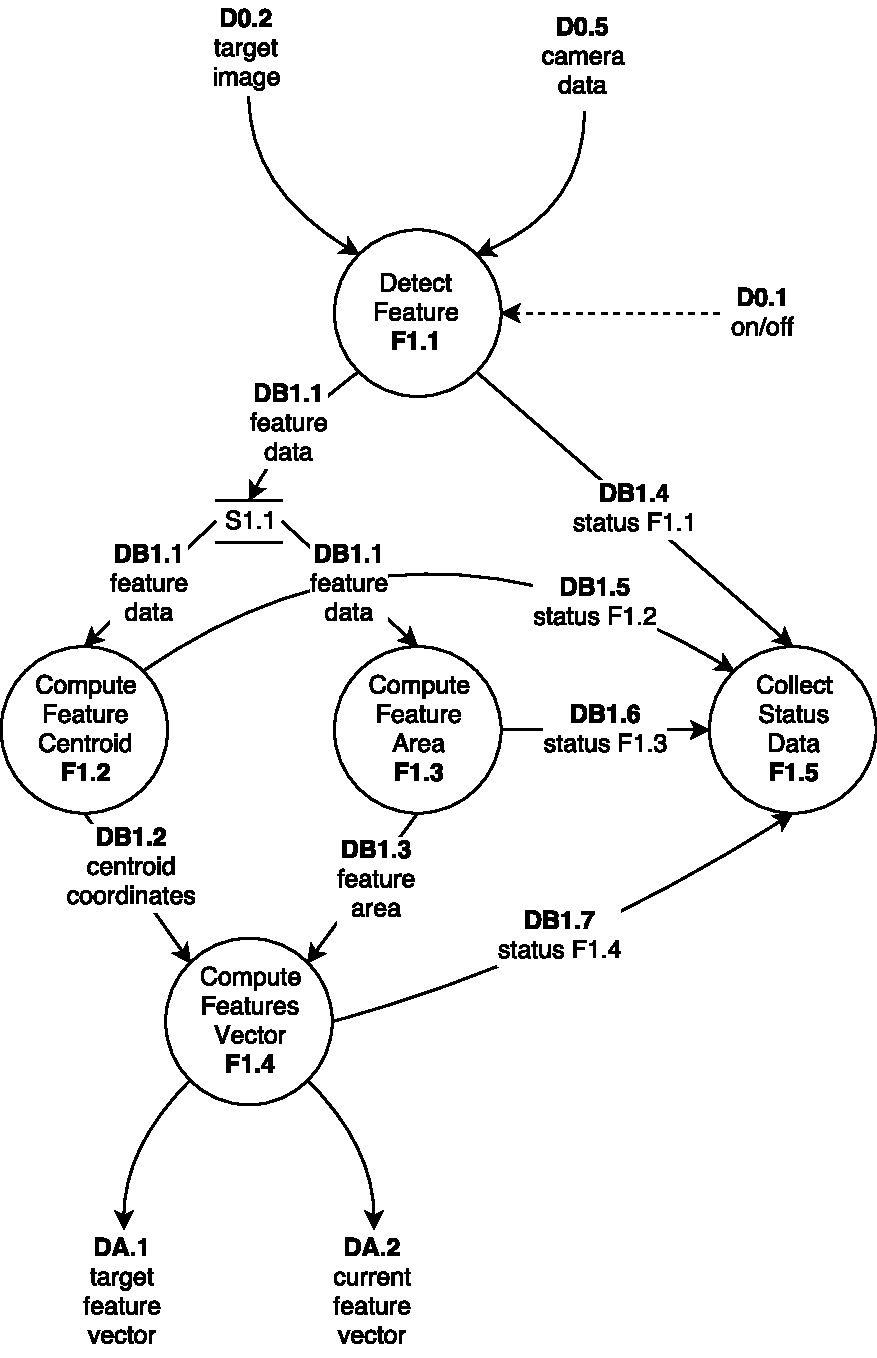
\includegraphics[width=0.9\textwidth]{content/chapter_03/images/sa_diagram_03.pdf}
	\caption{Data Flow Diagram - Level B1}
	\label{fig:sa_diag_03}
\end{figure}

\pagebreak

%%%%%%%%%%
\subsection{Level B2: Compute Current Visual Features}
\label{sec:level-B2}
%%%%%%%%%%

Figure \ref{fig:sa_diag_04} contains the Data Flow Diagram that describes the inner work of the process \textit{F2: Compute current visual features}.

\begin{figure}[!htb]
	\centering
	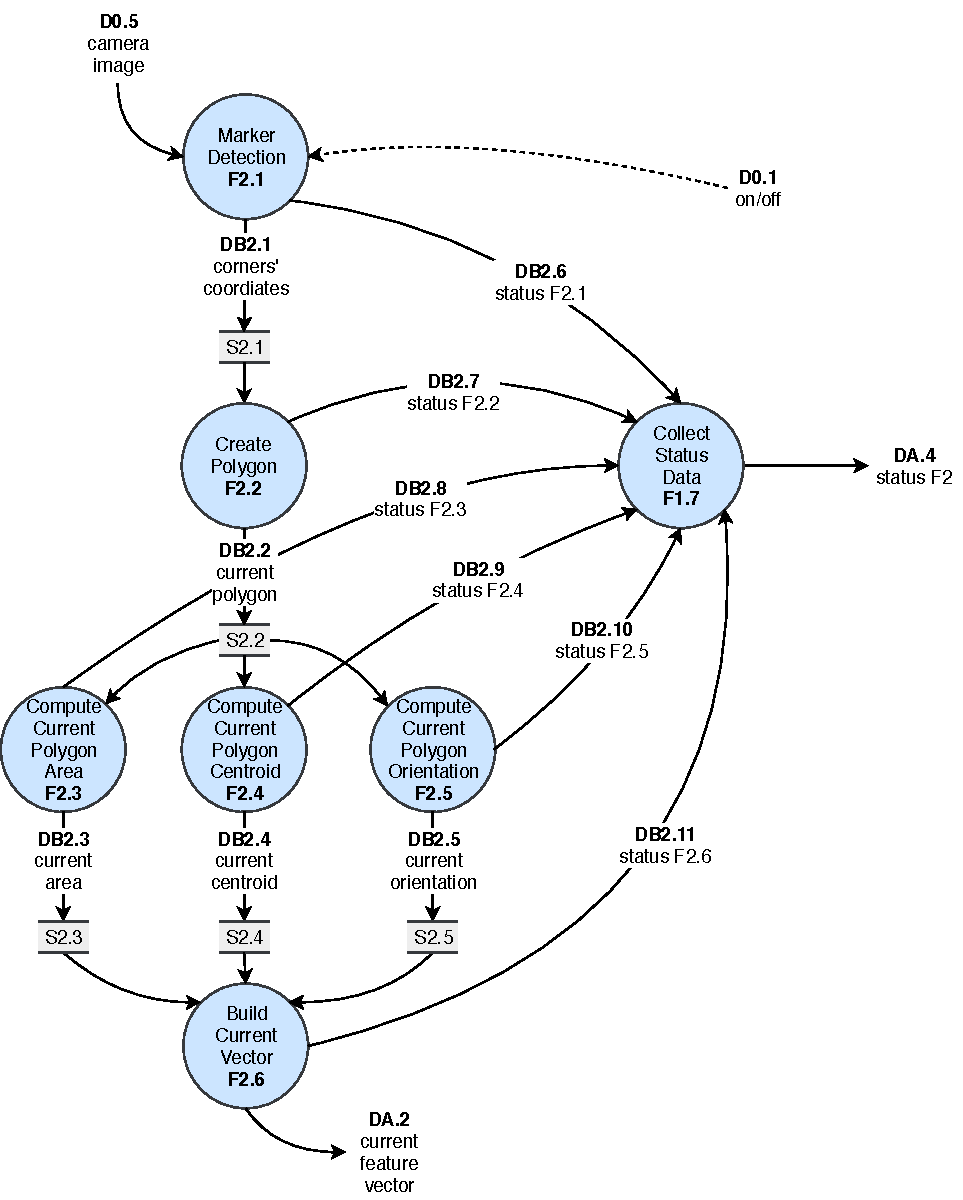
\includegraphics[width=0.9\textwidth]{content/chapter_03/images/sa_diagram_04.pdf}
	\caption{Data Flow Diagram - Level B2}
	\label{fig:sa_diag_04}
\end{figure}

\pagebreak

%%%%%%%%%%
\subsection{Level B4: Compute Control Law}
\label{sec:level-B3}
%%%%%%%%%%

Figure \ref{fig:sa_diag_05} contains the Data Flow Diagram that describes the inner work of the process \textit{F4: Compute control law}.

\begin{figure}[!htb]
	\centering
	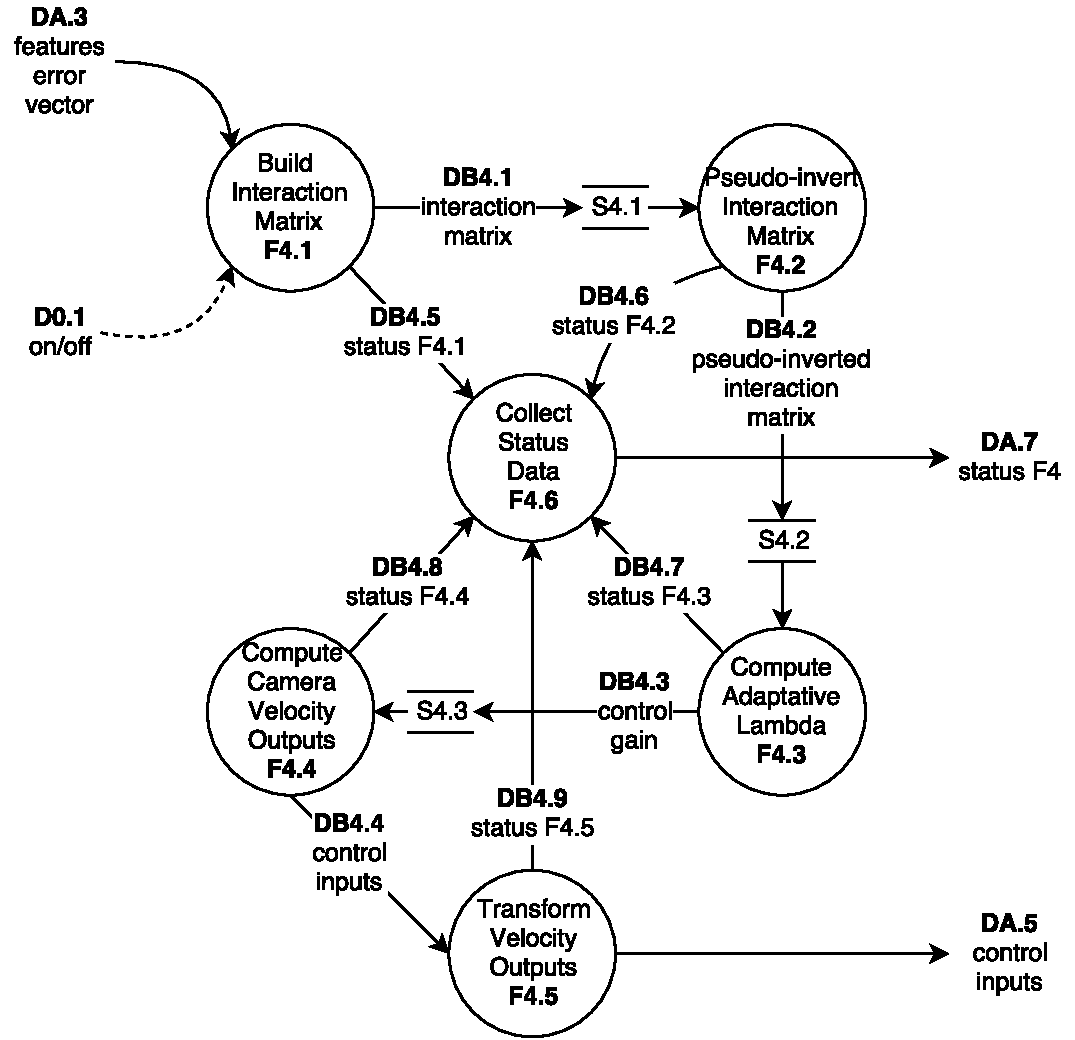
\includegraphics[width=\textwidth]{content/chapter_03/images/sa_diagram_05.pdf}
	\caption{Data Flow Diagram - Level B4}
	\label{fig:sa_diag_05}
\end{figure}

\pagebreak

\begin{table*}[!htb]
	\centering
	\begin{tabular}{lll}
		\toprule
		Flow & Type & Description \\
		\midrule
		DB1.1 & D & Vector containing the desired centroid coordinates for each blob\\
		DB1.2 & D & Desired polygon formed by the blobs \\
		DB1.3 & D & Desired polygon area \\
		DB1.4 & D & Desired polygon centroid coordinates\\
		DB1.5 & D & Desired polygon orientation angle \\
		DB1.6 & D & System status from process F1.1 \\
		DB1.7 & D & System status from process F1.2 \\
		DB1.8 & D & System status from process F1.3 \\
		DB1.9 & D & System status from process F1.4 \\
		DB1.10 & D & System status from process F1.5 \\
		DB1.11 & D & System status from process F1.6 \\
		\midrule
		DB2.1 & D & Vector containing the data from each of the detected blobs \\
		DB2.2 & D & Current polygon \\
		DB2.3 & D & Current area of the polygon \\
		DB3.4 & D & Current polygon centroid coordinates \\
		DB2.5 & D & Current polygon orientation angle \\
		DB2.6 & D & System status from process F2.1 \\
		DB2.7 & D & System status from process F2.2 \\
		DB2.8 & D & System status from process F2.3 \\
		DB2.9 & D & System status from process F2.4 \\
		DB2.10 & D & System status from process F2.5 \\
		DB2.11 & D & System status from process F2.6 \\
		\midrule
		DB4.1 & D & Visual Servoing interaction matrix \\
		DB4.2 & D & Pseudo-inverted Visual Servoing interaction matrix \\
		DB4.3 & D & Control gain $\lambda$ \\
		DB4.4 & D & Velocity control inputs in camera frame \\
		DB4.5 & D & System status from process F4.1 \\
		DB4.6 & D & System status from process F4.2 \\
		DB4.7 & D & System status from process F4.3 \\
		DB4.8 & D & System status from process F4.4 \\
		DB4.9 & D & System status from process F4.5 \\
		\bottomrule
	\end{tabular}
	\caption{Data Dictionary for Level B}
	\label{tab:DD-LB-a}
\end{table*}

\begin{table*}[!h]
	\centering
	\begin{tabular}{lll}
		\toprule
		Flow & Type & Description \\
		\midrule
		S1.1 & Datastore & Fixed frame to desired pose homogeneous transformation \\
		S1.2 & Datastore & Desired centroid coordinates for each blob \\
		S1.3 & Datastore & Desired target polygon \\
		S1.4 & Datastore & Desired polygon area \\
		S1.5 & Datastore & Desired polygon centroid coordinates \\
		S1.6 & Datastore & Desired polygon orientation angle \\
		S2.1 & Datastore & Blob edges, gray level and centroid coordinates \\
		S2.2 & Datastore & Current target polygon  \\
		S2.3 & Datastore & Current polygon area \\
		S2.4 & Datastore & Current polygon centroid coordinates \\
		S2.5 & Datastore & Current polygon orientation angle \\	
		S4.1 & Datastore & Visual servoing interaction matrix \\	
		S4.2 & Datastore & Pseudo-inverted Visual Servoing interaction matrix \\
		S4.3 & Datastore & Control gain $\lambda$ \\
		\bottomrule
	\end{tabular}
	\caption{Datastore Dictionary for Level B}
	\label{tab:DD-LB-b}
\end{table*}

\pagebreak

%%%%%%%%%%
\subsection{Level C1: Blob Detection and Tracking}
\label{sec:level-C1}
%%%%%%%%%%

Figure \ref{fig:sa_diag_06} contains the Data Flow Diagram that describes the inner work of the process \textit{F2.1: Blob detection and tracking}.

\begin{figure}[!htb]
	\centering
	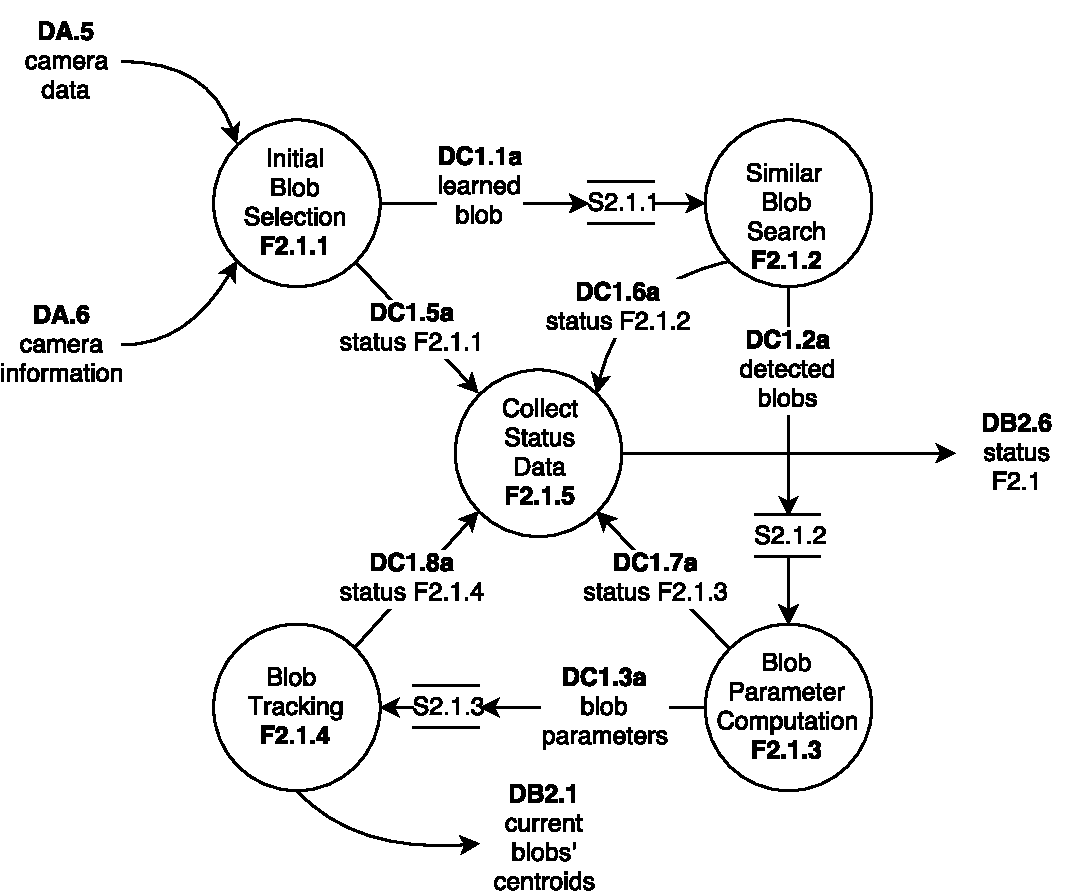
\includegraphics[width=\textwidth]{content/chapter_03/images/sa_diagram_06.pdf}
	\caption{Data Flow Diagram - Level C1}
	\label{fig:sa_diag_06}
\end{figure}

\begin{table*}[!htb]
	\centering
	\begin{tabular}{lll}
		\toprule
		Flow & Type & Description \\
		\midrule
		DC1.1a & D & Parameters of the initial blob \\
		DC1.2a & D & Vector containing the detected blobs \\
		DC1.3a & D & Vector containing the parameters of the detected blobs \\
		DC1.4a & D & Parameters of the initial blob \\
		DC1.5a & D & System status from process F2.1.1 \\
		DC1.6a & D & System status from process F2.1.2 \\
		DC1.7a & D & System status from process F2.1.3 \\
		DC1.8a & D & System status from process F2.1.4 \\
		\midrule
		S2.1.1 & Datastore & Blob edges, gray level and centroid coordinates \\
		S2.1.2 & Datastore & Blob edges, gray level and centroid coordinates \\
		S2.1.3 & Datastore & Blob centroid coordinates and area \\
		\bottomrule
	\end{tabular}
	\caption{Data Dictionary for Level C}
	\label{tab:DD-LC}
\end{table*}
                              
\end{document}